\documentclass{beamer}
\usepackage{times}
\usepackage[utf8]{inputenc}
\usepackage[czech]{babel}
\usepackage{times}
\usepackage{graphicx}
\usepackage{url}

\providecommand{\uv}[1]{\quotedblbase#1\textquotedblleft}

\renewcommand{\UrlFont}{\normalsize}

\title{Vývoj číslic}
\date{\today}
\author{Ondřej Valeš}

\begin{document}

\frame{\titlepage}

\frame{\frametitle{Obsah} \tableofcontents}

\section{Vznik}

\begin{frame}
	\frametitle{Vznik číslic}
	\begin{itemize}
		\item Potřeba sdělit informace o~počtu, množství		
		\begin{itemize}
			\item Lov (z~kolika zvířat se tlupa nají)
			\item Obchod (kolik kůží chci vyměnit)
			\item Boj (je druhá tlupa větší)
		\end{itemize}
		\item Počítání objektů, reprezentace stejným možstvím kamínků
		\item Počítání na prstech, gesta ruky
		\item Abstrakce, počet zářezů na kosti, číslice
	\end{itemize}
\end{frame}

\begin{frame}
	\frametitle{Místa vzniku}
	\begin{itemize}
		\item Nezávisle na více místech		
		\begin{itemize}
			\item Blízký východ
			\item Dálný východ
			\item Střední amerika
		\end{itemize}
	\end{itemize}
	\begin{figure}[h]
		\centering
		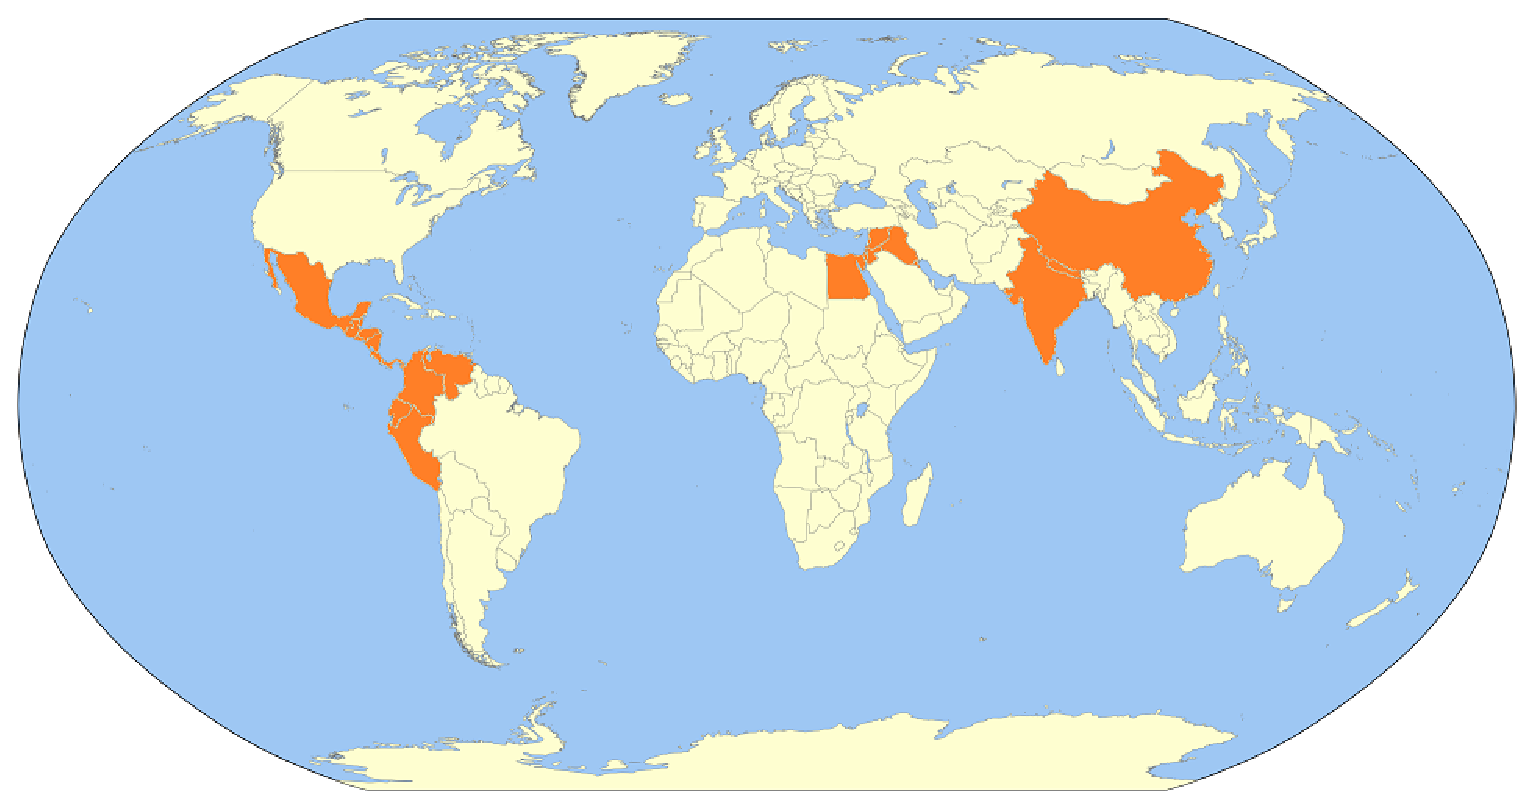
\includegraphics[width=\textwidth]{world}
	\end{figure}
\end{frame}

\section{Číslicové systémy}

\subsection{Sumerské číslice}
\subsection{Egyptské číslice}
\begin{frame}
	\frametitle{Blízký východ}
	\begin{itemize}
		\item Sumerské číslice
		\begin{itemize}
			\item Vznik přibližně 2000 ante
			\item Základ šedesát
			\item Symboly pro jedna a deset
		\end{itemize}
	\end{itemize}
	\begin{figure}[h]
		\centering
		$ 59 = $ 
\includegraphics[height=20pt]{sumer_59}
	\end{figure}
	\begin{itemize}
		\item Egyptské číslice
		\begin{itemize}
			\item Vznik přibližně 3000 ante
			\item Symboly pouze pro násobky desíti
			\item Zápis jiných čísel pomocí sčítání existujících smybolů
		\end{itemize}
	\end{itemize}
	
	\center{$ 312 = 100 + 100 + 100 + 10 + 1 + 1$}
	
	\begin{figure}[h]
		\centering
		\includegraphics[height=10pt]{hiero_100}
		\includegraphics[height=10pt]{hiero_100}
		\includegraphics[height=10pt]{hiero_100}
		\includegraphics[height=10pt]{hiero_10}
		\includegraphics[height=10pt]{hiero_1}
		\includegraphics[height=10pt]{hiero_1}
	\end{figure}
\end{frame}

\subsection{Číslice bráhmi}
\subsection{Čínské číslice}
\begin{frame}
	\frametitle{Dálný východ}
	\begin{itemize}
		\item Číslice bráhmi
		\begin{itemize}
			\item Vznik přibližně 300 ante
			\item Základ deset
			\item Symboly pro čísla od 1 do 9
			\item Číslice po 3 velmi podobné římským číslicím
			\item Předchůdce systému používaného dnes
		\end{itemize}
	\end{itemize}
	\begin{figure}[h]
		\centering
		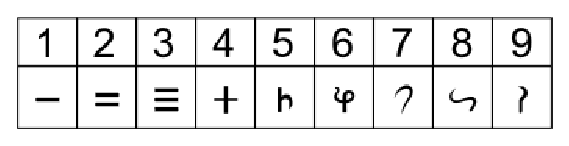
\includegraphics[height=25pt]{brahmi}
	\end{figure}
	\begin{itemize}
		\item Čínské číslice
		\begin{itemize}
			\item Vznik přibližně 1300 ante
			\item Podobný systému o~základu deset
			\item Ruzné symboly pro opakující se hodnoty (desítky, stovky,\,\dots)
		\end{itemize}
	\end{itemize}
\end{frame}

\begin{frame}
	\frametitle{Ukázka čínských symolů}
	\begin{figure}[h]
		\centering
		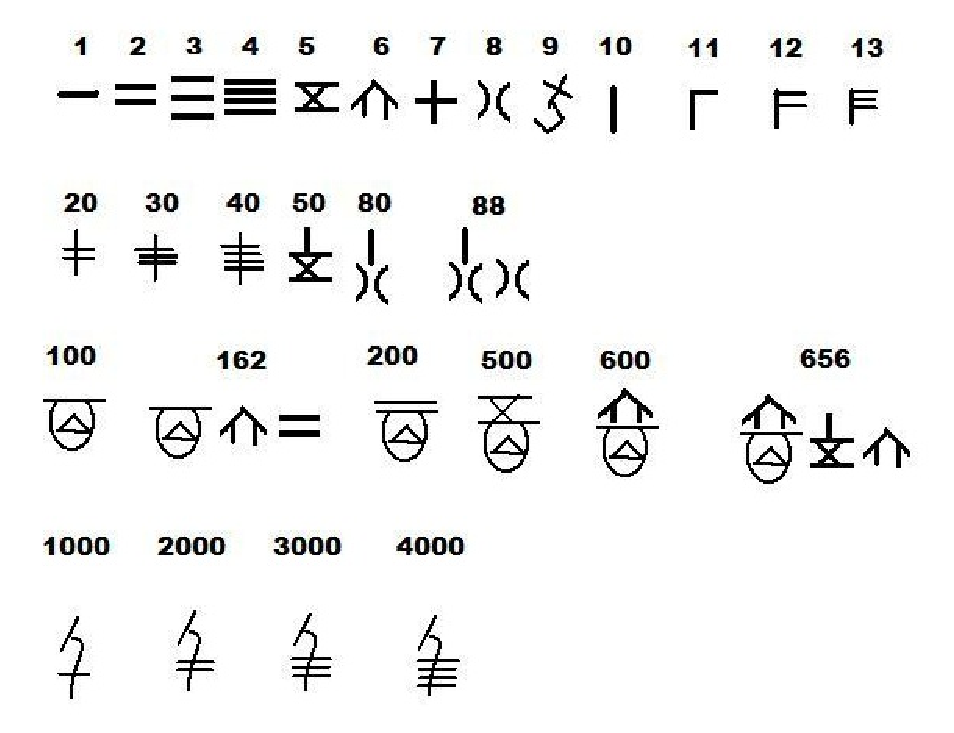
\includegraphics[width=\textwidth]{sino}
	\end{figure}
\end{frame}

\subsection{Mayské číslice}
\begin{frame}
	\frametitle{Střední amerika}
	\begin{itemize}
		\item Mayské číslice
		\begin{itemize}
			\item Vznik přibližně 200 ante
			\item Základ dvacet
			\item Symboly pro jedničku a pětku
			\item V~principu velmi podobný systému používanému dnes
		\end{itemize}
	\end{itemize}
	\begin{figure}[h]
		\centering
		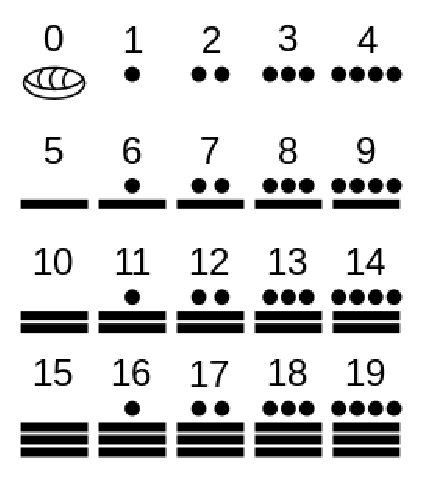
\includegraphics[width=80pt]{maya}
	\end{figure}
\end{frame}

\section{Současné systémy}
\begin{frame}
	\frametitle{Současné systémy}
	\begin{itemize}
		\item Římské číslice
		\begin{itemize}
			\item Vznik přibližně 800 ante
			\item Symboly podobné gestům ruky
		\end{itemize}
	\end{itemize}
	\begin{figure}[h]
		\centering
		
\includegraphics[width=60pt]{roman}
	\end{figure}
	\begin{itemize}
		\item Arabské číslice
		\begin{itemize}
			\item Vznik přibližně 400 ante v~Indii
			\item V~evropě od přibližně od roku 1000
		\end{itemize}
	\end{itemize}
	\begin{figure}[h]
		\centering
		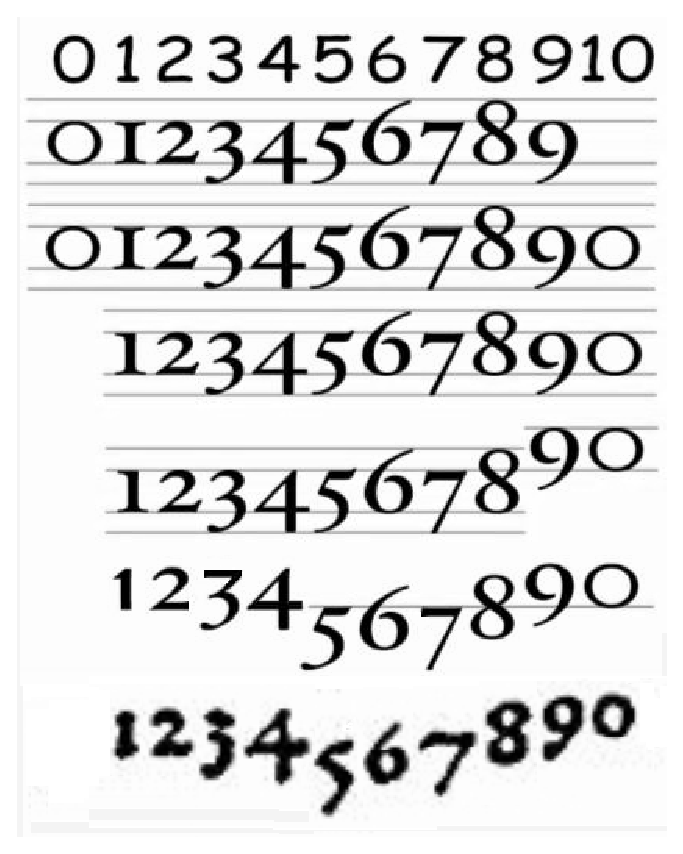
\includegraphics[width=60pt]{arabic}
	\end{figure}
\end{frame}

\section{Zdroje}
\begin{frame}
	\frametitle{Zdroje}
	\begin{itemize}
		\item Zápis čísel v~různých kulturách\\
		\url{www.freeside.cz/monika/zapis_cisel/indove.html}
		\item Psaní čísel\,--\,CINSTINA.CZ
		\url{www.cinstina.cz/article-writing-chinese-numbers.html}
		\item History of ancient numeral systems\,--\,Wikipedia
		\url{en.wikipedia.org/wiki/History_of_ancient_numeral_systems}
	\end{itemize}
\end{frame}

\end{document}